\documentclass[a4paper,12pt]{article}
\usepackage[a4paper,top=1.3cm,bottom=2cm,left=1.5cm,right=1.5cm,marginparwidth=0.75cm]{geometry}
\usepackage{setspace}
\usepackage{cmap}
\usepackage{mathtext}
\usepackage[T2A]{fontenc}
\usepackage[utf8]{inputenc}
\usepackage[english,russian]{babel}
\usepackage{multirow}
\usepackage{graphicx}
\usepackage{wrapfig}
\usepackage{tabularx}
\usepackage{float}
\usepackage{longtable}
\usepackage{hyperref}
\hypersetup{colorlinks=true,urlcolor=blue}
\usepackage[rgb]{xcolor}
\usepackage{amsmath,amsfonts,amssymb,amsthm,mathtools}
\usepackage{icomma}
\mathtoolsset{showonlyrefs=true}
\usepackage{euscript}
\usepackage{mathrsfs}
\usepackage{float}
\setlength{\parindent}{1.5cm} % Устанавливает отступ в 1.5 см для всех абзацев


\DeclareMathOperator{\sgn}{\mathop{sgn}}
\newcommand*{\hm}[1]{#1\nobreak\discretionary{}
	{\hbox{$\mathsurround=0pt #1$}}{}}

\title{\textbf{Отчёт о выполненой лабораторной работе \\ \textit{Измерение удельной теплоёмкости воздуха при постоянном давлении (2.1.1)}}}
%\title{\textit{}{Измерение удельной теплоёмкости воздуха при постоянном давлении (2.1.1)}}
\author{Каплин Артём Б01-402}
\date{15 февраля 2025}

\begin{document}

\maketitle

	\section{Аннотация}

	\textbf{Цель работы:} измерить повышение температуры воздуха в зависимости от мощности
подводимого тепла и расхода при стационарном течении через трубу; исключив тепловые потери, по результатам измерений определить теплоёмкость воздуха при постоянном давлении.\\
\newline
	\textbf{Оборудование:} теплоизолированная стеклянная трубка; электронагреватель; источник питания постоянного тока; амперметр, вольтметр (цифровые мультиметры); термопара, подключенная к микровольтметру; компрессор; газовый счётчик;
секундомер.

	\section{Теоретические сведения}

        Измерение теплоёмкости тел обычно производится в калориметрах, в которых регистрируется изменение его температуры \(dT\) в зависимости от кол-ва теплоты \(\delta{Q}\) , полученного телом. Теплоёмкость тела в некотором процессе определяется как их соотношение:

        \[C = \frac{\delta{Q}}{dT}\]

        Надёжность в основном определяется качеством калориметра. Необходимо, чтобы кол-во тепла, затрачиваемое на нагревание тела, существенно превосходило тепло, расходуемое на нагревание калориметра, а также на потери тепла из установки. При измерении теплоёмкости газов выполнить эти требования довольно сложно.  Для увеличения количества нагреваемого газа при неизменных размерах установки в нашей работе исследуемый газ (воздух) продувается через калориметр, внутри которого установлен нагреватель. При этом
        измеряются мощность нагревателя, масса воздуха, протекающего в единицу
        времени (расход), и приращение его температуры.

        Рассмотрим газ, протекающий стацианарно слева направо через трубу постояного сечения, в которой установлен нагревательный элемент. Пусть за некоторый момент времени \(dt\) прошла малая порция газа \(dm = q dt\)  , где \(q\) --- \textit{массовый расход} газа в трубе. 

        \begin{wrapfigure}{r}{0.4\textwidth} % {r} - выравнивание по правому краю, 0.4\textwidth - ширина изображения
            \centering
            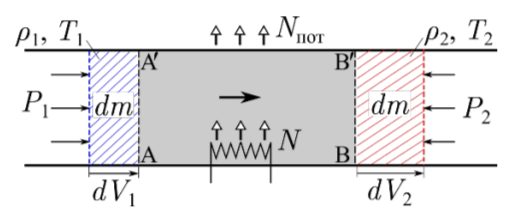
\includegraphics[width=0.4\textwidth]{211kal.png} % замените на ваш путь к изображению
        \end{wrapfigure}

        Псть \textit{мощность нагревательного элемента} \(N\), а мощность потерь на обмен с окружающей средой \(N_{\text{пот}}\), тогда имеем:

        \[\delta Q = (N - N_{\text{пот}})dt = c \cdot dm \cdot \Delta T\] \\

        Таким образом, при малом расходе и достаточно большом диаметре трубы перепад давления мал, т.е. будет равен \(P_{0}\) --- атмосферному давлению. Тогда формула принимает вид:

        \[c_p = \frac{N - N_{\text{пот}}}{q\Delta T}\]

        \section{Течение газа по трубе}

        \underline{Запишем уравнение Бернули (m = 1 кг):} 
        \[\frac{v^2}{2} + \frac{p}{\rho} + u^{\text{уд}} = const\]

        , где \(u^{\text{уд}}\) --- внутренняя энергия газа. Введём \(i = \frac{p}{\rho} + u^{\text{уд}}\) --- \textit{удельная энтальпия газа}.\\

        Наконец, пусть \(\delta Q\) — количество тепла, суммарно полученное газом в рассматриваемой области — включая тепло от нагревателя, теплопередачу через стенки и торцы, тепловыделение при трении и т.д. В стационарном состоянии энергия газа, заполняющего калориметр, неизменна, поэтому

        \[\left(i_2 - i_1 + \frac{v^2_{1}}{2} - \frac{v^2_{1}}{2} \right)dm = \delta Q \]

        Данное cоотношение справедливо для любой стационарно текущей непрерывной среды и представляет собой обобщение известного уравнения Бернулли,
        учитывающее выделение и потери тепла. Оно справедливо при условии, что
        в системе устанавливается не только стационарное течение, но и стационарное распределение температуры. Последнее весьма важно для нашего опыта,
        поскольку время установления может быть довольно велико.

        Если предположить, что кинетическая энергия течения мала по сравнению с энергией нагрева (\(dK<< \delta Q\)), то получим 
        \[(i_2 - i_1)dm = \delta Q\]

        то есть полученное газом тепло идёт на приращение энтальпии.

        Итак, более подробное рассмотрение позволяет установить, что предыдущая формула справедлива даже в том случае, если перепад давлений на концах трубы не мал, при условии, что газ можно считать идеальным , а его кинетической энергией можно пренебречь.
       
        \section{Экспериментальная установка}

        Схема установки изображена на рис.  Воздух, нагнетаемый компрессором, прокачивается через калориметр. Калориметр представляет собой стеклянную цилиндрическую трубку с двойными стенками, запаянными с торцов. На внутреннюю поверхность стенок трубки нанесено серебряное покрытие для минимизации потерь тепла за счет излучения. Воздух из пространства между стенками калориметра откачан до высокого вакуума  для минимизации потерь тепла, обусловленных теплопроводностью.

        Нагреватель в виде намотанной на пенопласт нихромовой проволоки расположен внутри калориметра непосредственно в воздушном потоке. Нагрев
        проволоки производится от регулируемого источника постоянного тока (ИП).
        Напряжение \(U\) на нагревателе и ток \(I\) через него регистрируются цифровыми
        мультиметрами. Таким образом, мощность нагрева равна

        \[N = UI\]

        \begin{center}
		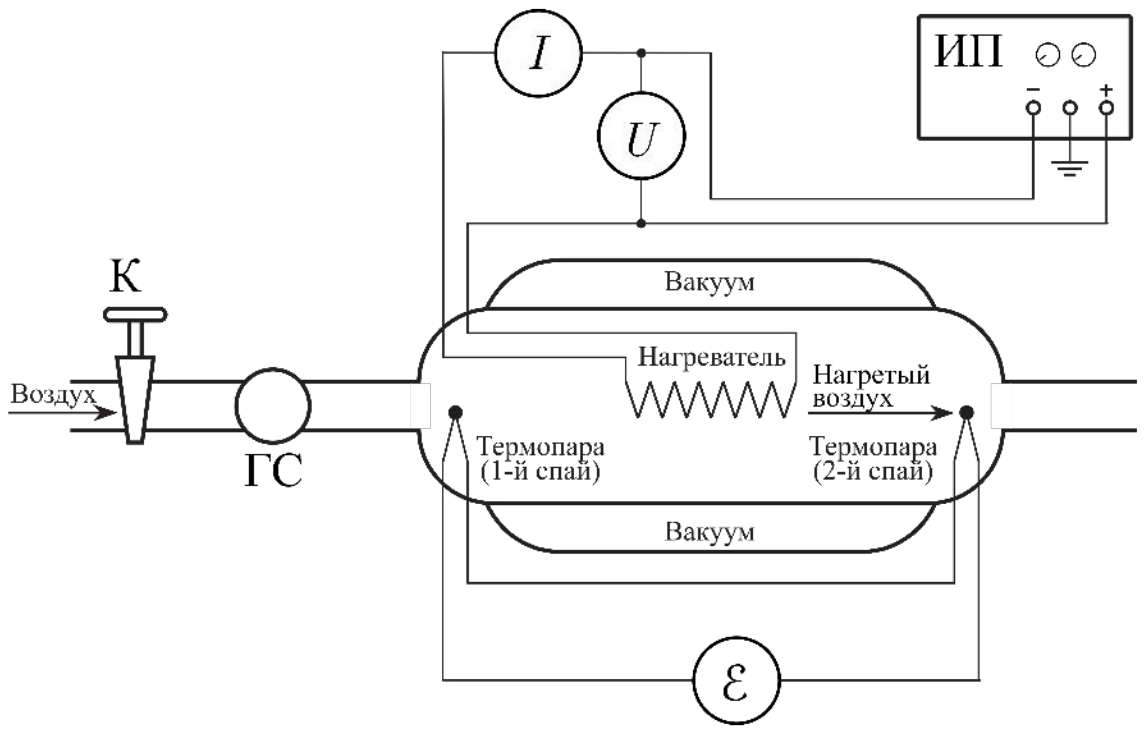
\includegraphics[width=0.7\textwidth]{asd.png}
	\end{center}

        Для измерения разности температур \(\Delta T\) служит медно-константановая
        термопара. Один спай термопары расположен в струе воздуха, входящего в
        калориметр, и находится при комнатной температуре, а второй — в струе выходящего нагретого воздуха. Константановая проволока термопары расположена внутри калориметра, а медные проводники подключены к цифровому
        вольтметру. Возникающая в термопаре ЭДС \(\mathcal{E}\) пропорциональна разности
        температур \(\Delta T\) спаев:

        \[\mathcal{E} = \beta \Delta T,\]
        где $\beta = 40,7 \frac{\text{мкВ}}{^\circ C}$ --- чувствительность медно-константановой термопары в рабочем диапазоне температур (20–30 ℃). ЭДС регистрируется с помощью микровольтметра.\\

        
        Объём воздуха, прошедшего через калориметр, измеряется газовым счётчиком ГС. Для регулировки расхода служит кран К. Время \( \Delta t \) прохождения некоторого объема \( \Delta V \) воздуха измеряется секундомером. Объёмный расход равен \( \frac{\Delta V}{\Delta t} \), массовый расход может быть найден как
        \[
        q = \rho_0 \frac{\Delta V}{\Delta t},
        \]
        где \( \rho_0 \) — плотность воздуха при комнатной температуре, которая в свою очередь может быть получена из уравнения Менделеева–Клапейрона:
        \[
        \rho_0 = \frac{\mu P_0}{RT_0},
        \]
        где \( P_0 \) — атмосферное давление, \( T_0 \) — комнатная температура (в Кельвинах), \( \mu = 29,0 \, \text{г/моль} \) — средняя молярная масса (сухого) воздуха.
        
        Учитывая особенности устройства калориметра, следует ожидать, что мощность нагревателя расходуется не только на нагрев массы прокачиваемого воздуха, но и частично теряется за счет нагрева внутренних стенок термостата и рассеяния тепла через торцы термостата. Можно предположить, что при небольшом нагреве (\( \Delta T \ll T_0 \)) мощность потерь тепла \( N_{\text{пот}} \) прямо пропорциональна разности температур:
        \[
        N_{\text{пот}} = \alpha \Delta T,
        \]
        где \( \alpha \) — некоторая константа. При этом условии основное соотношение (2) принимает вид
        \[
        N = (c_P q + \alpha) \Delta T.
        \]
        \newpage

        \section{Обработка результатов}

        \begin{enumerate}
		\item Подготовим к работе газовый счетчик: проверим корректность работы: убедимся, что при постоянном расходе его стрелка вращается равномерно. Включим вольтметр,
        предназначенный для измерения ЭДС термопары и проверим, что напряжение на термопаре равно нулю.
		
		\item Запишем показания комнатной температуры и давления. $$T_{0} = 23,4 \pm 0,4 \; ^\circ C, \quad P_{0} = 101180 \pm 300 \, \text{Па} $$
        \[\varepsilon_T = 1,71 \% \quad \quad \varepsilon_P = 0,3 \%\]
        
            \item Посчитаем плотность воздуха 
            \[
            \rho_0  = \frac{P_0\mu}{RT_0} = 1, 1897 \frac{\text{г}}{\text{м}^3}
            \]
            \[\varepsilon_{\rho} = \sqrt{\varepsilon^2_T + \varepsilon^2_P} = 1,74 \% \]

		\item Установим максимальный расход воздуха на газовом счётчике (класс точности --- 1,0) -- $5$л за $30 $с. Определим массовый расход воздуха $q_{0}$ [г/с].
		
		\[q_1 = \rho_0 \frac{\Delta V}{\Delta t} = 0,1879 \frac{\text{г}}{\text{с}} \quad  \quad \varepsilon_q = 2,0 \%\]

            Повторим измерения для втрого расхода: \(q_2 = ≈ 0, 1054 \frac{\text{г}}{\text{с}}\)

            \item Считая воздух идеальным двухатомным газом, определим теоретическую удельную теплоёмкость при постоянном давлении по следующим формулам:

            \[
            C_v = \frac{5R}{2\mu} = 0,72 \, \frac{\text{Дж}}{\text{г} \cdot \text{К}}  \quad \quad C_p = C_v + \frac{R}{\mu} = 1,0034 \frac{\text{Дж}}{\text{г} \cdot \text{К}} \quad \quad 
            \]
            
		\item Оцените величину тока нагревателя $I_0$, требуемого для нагрева воздуха
            на $\Delta T = 1K$ по следующим формулам:

            \[
                 \quad N_{min} = C_pq_0\Delta T = 0,189 \, \text{Вт}
            \]
                Сопротивление проволоки нагревателя $R_{\text{н}} = 37 \quad \text{Ом}$
            \[I_{min} = \sqrt{\frac{N_{min}}{R_{\text{н}}}} = 71,47 \,\text{мА}\]
            \item  Запишем погрешности у приборов:
                \begin{itemize}
                    \item Погрешностью напряжения на термопаре  $\varepsilon_{\mathcal{E}} = 0,004 \%$
                    \item Погрешность на амперметре $\varepsilon_I = 0,2 \%$
                    \item На вольтметре $\varepsilon_u = 0,03 \%$
                \end{itemize}
            \[
            \sigma_N = \bar{N} \cdot \sqrt{\left( \frac{\sigma_I}{\bar{I}} \right)^2 + \left( \frac{\sigma_U}{\bar{U}} \right)^2} = 0,0003
            \]

		
	\end{enumerate}

        Запишем измерения расхода воздуха:\\

        При расходе $q_1$:
        \begin{figure}[H]
        \center
        \begin{tabular}{|c|c|c|c|c|c|c|}\hline
        {} &   $\mathcal{E}, \text{мкВ}$ & $U, \text{В}$ & $I, \text{мА}$ & $\Delta T, K$ & $N,\, \text{Вт}$ & $R_\text{н},\ \text{Ом}$ \\\hline
        1 &  39  &  2,50 &  71,27  &   0,96 &  0.18 &  35,44 \\\hline
        2 &  76  &  3,62 &  101,14 &   1,87 &  0.37 &  36,17 \\\hline
        3 &  143 &  5,05 &  141,30 &  3,51  &  0,71 &  35,56 \\\hline
        4 &  217 &  6,27 &  175,38 &  5,33 &  1,10 &  35,76\\\hline
        5 &  283 &  6,96 &  199,90 &  6,95 &  1,39 &  34,78 \\\hline
        6 &  350 &  7,78 &  223,40 &  8,60 &  1,74 &  34,86 \\\hline
        \end{tabular}
        \end{figure}

        При расходе $q_2$:
        \begin{figure}[H]
        \center
        \begin{tabular}{|c|c|c|c|c|c|c|}\hline
        {} &   $\mathcal{E}, \text{мкВ}$ & $U, \text{В}$ & $I, \text{мА}$ & $\Delta T, K$ & $N,\, \text{Вт}$ & $R_\text{н},\ \text{Ом}$ \\\hline
        1 &  36  &  1,90 &  155.8 &  0,88 &  0,11 &  35,46 \\\hline
        2 &  82  &  2,98 &  182.7 &  2,01 &  0.25 &  36,13 \\\hline
        3 &  162 &  4,20 &  206.7 &  3,98 &  1.49 &  35,41 \\\hline
        4 &  241 &  5,16 &  226.8 &  5,92 &  0,74 &  35,69 \\\hline
        5 &  324 &  5,95 &  245.7 &  7,96 &  0,99 &  35,84 \\\hline
        6 &  405 &  6,67 &  223,4 &  9,93 &  1,24 &  35,78 \\\hline
        \end{tabular}
        \end{figure}

        
        \subsection{Построим графики по МНК}
        \textbf{Для первой серии опытов:}  $k_1 = 4,911 \pm 0,049  (\varepsilon = 0,99 \%)$
        \begin{center}
		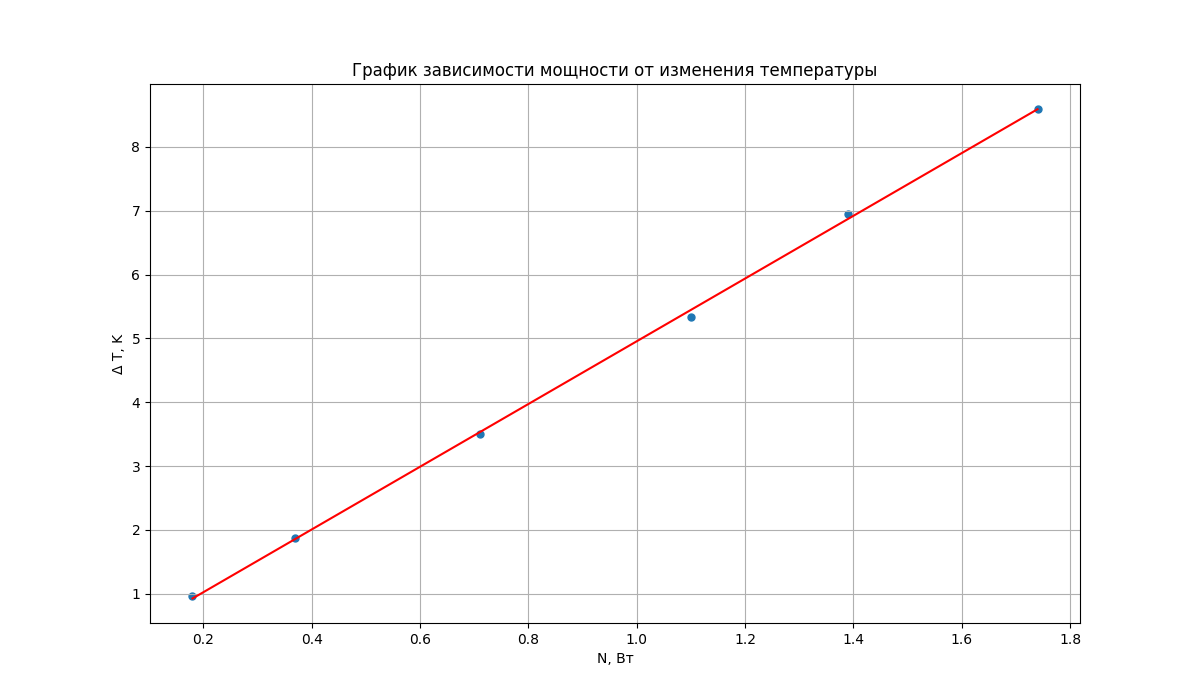
\includegraphics[scale=0.6]{q1.png}
	\end{center}
        \textbf{Для второй серии опытов:}  $k_2 = 8,021 \pm 0,023  (\varepsilon = 0,29 \%)$

        \begin{center}
		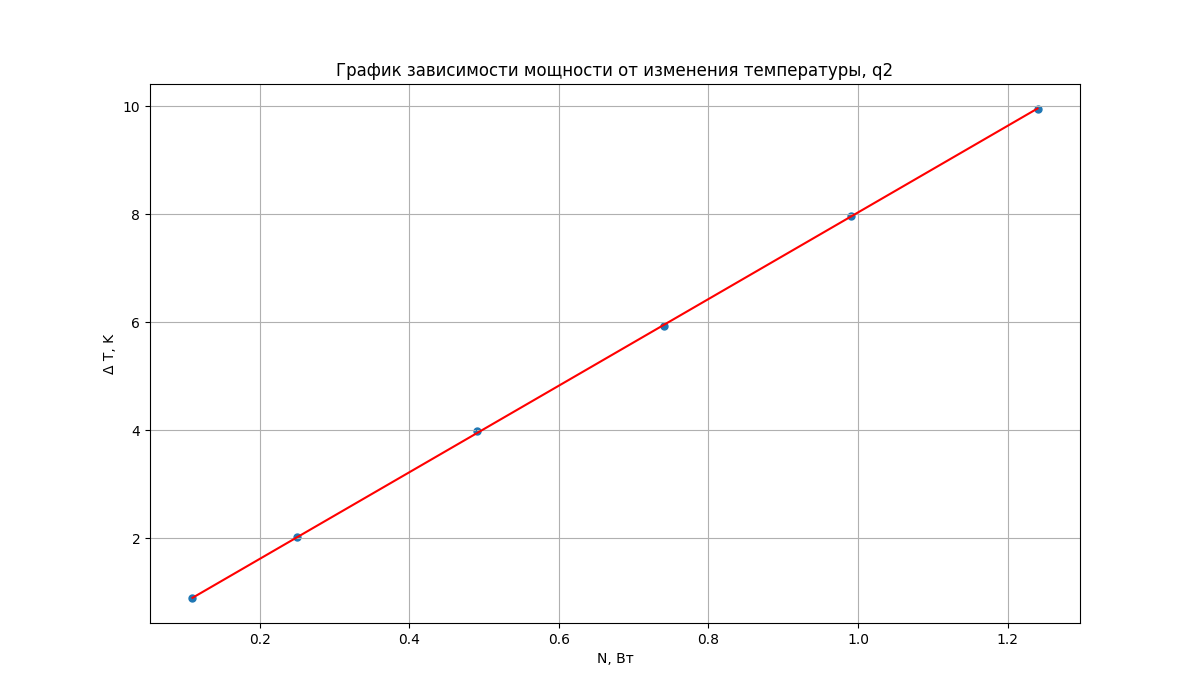
\includegraphics[scale=0.6]{q2.png}
	\end{center}

        Найдём $c_p$ и $\alpha$ из системы уравнений:

        \[
        \begin{aligned}
            \begin{cases}
                \displaystyle c_P = \frac{k_2 - k_1}{(q_1 - q_2)\, k_1\, k_2} \\[10pt]
                 \displaystyle \alpha = \frac{k_2-k_1-c_P(q_1+q_2)}{2\,k_1\,k_2}
            \end{cases} 
            \quad & \text{и} \quad
            \begin{cases}
                 \displaystyle c_P = 0,957 \pm 0,021\ \frac{\text{Дж}}{\text{г  К}} (\varepsilon_{c_p} = 2,25 \%) \\[10pt]
                 \displaystyle \alpha = 0,0359 \pm 0,0011\ \frac{\text{Вт}}{K} (\varepsilon_{\alpha} = 3,18  \%)
            \end{cases}
        \end{aligned}
        \]

        \subsection{Посчитаем долю тепловых потерь}

        \begin{table}[H]
        \centering
        \caption{Доля тепловых потерь}
        \begin{tabular}{|c|c|}
        \hline
         1 серия опытов $\frac{N_{pot}}{N}$   & 2 серия опытов $\frac{N_{pot}}{N}$ \\ \hline
            0,1917            & 0,2873 \\ \hline
        0,1814     & 0,2888 \\ \hline
        0,1775     & 0,2916 \\ \hline 
        0,1739       & 0,2872 \\ \hline
        0,1795 & 0,2887 \\ \hline
        0,1774       & 0,2881 \\ \hline
        \end{tabular}
    \end{table}

    \subsection{Подведём итоги}

    Сравним полученное значение удельной теплоёмкости с табличным (сухого воздуха при давлении 1 атм)

    \begin{table}[H]
    \centering
    \caption{Сравнение}
    \begin{tabular}{|c|c|c|c|}
        \hline
                  & $c_p$, Дж/г·K & $\Delta c_p$, Дж/г·K & $\varepsilon_{c_p}$, \% \\
        \hline
        экспериментальное & 0,957 & 0,021 & 2,25 \\
        \hline
        теоретическое    & 1,003 & 0,046 & 4,6 \\
        \hline
        табличое          & 1,006 & 0,049 & 4,9 \\
        \hline
    \end{tabular}
    \caption{Таблица 5: Сравнение характеристик различных материалов}
\end{table}


    \section{Выводы}
    В ходе лабораторной работы мы измерили зависимость повышение температуры воздуха от мощности подво-
димого тепла и расхода при стационарном течении через трубу. Также определили теплоёмкость воздуха при постоянном давлении.
Результат отличается от табличного примерно на 5\% . Такое расхождение могло получиться из-за того что мы брали модель воздуха, как идеальный двухатомный газ. Также свой вклад в порешность внесли приборы. Для установления равновесия в системе необходимо, чтобы прошло большое количество времени, что также могло повлиять на неточность результата. Также можно заметить, что потери увеличиваются с увеличением расхода воздуха.
\end{document}